\section{Chapter 7 -- Generics and Collections}
\subsection{Methods of Class Object Covered on the Exam}
\begin{center}
\begin{tabular}{lp{.6\textwidth}}
    \textbf{Method} & \textbf{Description} \\
    \hline
    \verb#boolean equals(Object o)# & Determines whether two objects are 
    meaningfully equivalent \\
    \verb#void finalize()# & Called by garbage collector when it sees that the 
    object cannot be referenced \\
    \verb#int hashcode()# & Returns a hashcode value for an object, so that the 
    object can be used in \verb#Collection# classes that use hashing, including 
    \verb#Hashtable#, \verb#HashMap# and \verb#HashSet# \\
    \verb#final void notify()# & Wakes up a thread that is waiting for this 
    object's lock \\
    \verb#final void notifyAll()# & Wakes up all threads that are waiting for 
    this object's lock \\
    \verb#final void wait()# &  Causes the current thread to wait until another 
    thread calls \verb#notify()# or \verb#notifyAll()# on this object \\
    \verb#String toString()# & Returns a String representation of the object \\
\end{tabular}
\end{center}

\subsection{Overriding hashCode(), equals() and toString()}
\subsubsection{The toString() method}
Override \verb#toString()# when you want to create a meaningful String 
representing the objects of a class. If \verb#tostring()# is not overridden, 
\verb#Object#'s version returns the class name followed by the \verb#@# symbol, 
and then the unsigned hexadecimal representation of the object's hashcode

\subsubsection{Overriding equals()}
When you need to know if two references are identical, use \verb#==#, but when 
you need to know if the two objects themselves (not the references) are 
meaningfully equal, use the \verb#equals()# method

\subsubsection{If equals() is not Overridden}
\verb#Obejcts#'s \verb#equals()# method uses only the \verb#==# operator for 
comparisons, so unless you override \verb#equals()#, two objects are considered 
equal only if the two references refer to the same object. If you don't 
override the \verb#equals()# method, you will not be able to use those objects 
as a key in a hashtable and you probably will not get accurate Sets, such that 
there are no conceptual duplicates. The bottom line is: if you want objects of 
your class to be used as keys for a hashtable (or as elements in any data 
structure that uses equivalency for searching and/or retrieving an object), 
then you must override \verb#equals()# so that two different instances can be 
considered the same

\subsubsection{Implementing an equals() Method}
Logically, there are two things we have to do in order to make a valid equality 
comparison:
\begin{itemize}
    \item Ensure the object being tested is of the correct type
    \item Compare the attributes we decide will determine equality
\end{itemize}

\subsubsection{The equals() Contract}
\begin{itemize}
    \item It is reflexive -- for any non-null reference \verb#x#, \verb#x.equals(x)# 
    should return \verb#true#
    \item It is symmetric -- for any non-null reference values \verb#x# and \verb#y#, 
    \verb#x.equals(y)# should return \verb#true# iff \verb#y.equals(x)# returns 
    \verb#true#
    \item It is transitive -- for any non-null reference values \verb#x#, \verb#y# and 
    \verb#z#, if \verb#x.equals(y)# returns \verb#true# and \verb#y.equals(z)# 
    returns true, then \verb#x.equals(z)# returns \verb#true#
    \item It is consistent -- for any non-null reference values \verb#x# and \verb#y#, 
    multiple invocations of \verb#x.equals(y)# consistently return the same 
    value, provided no information used in the comparison is modified
    \item For any non-null reference value \verb#x#, \verb#x.equals(null)# 
    should return \verb#false#
\end{itemize}
\verb#equals()# and \verb#hashCode()# are bound together by a joint contract 
that specifies if two objects are considered equal using \verb#equals()#, then 
they must have identical hashcode values. So to be safe, if you override 
\verb#equals()#, override \verb#hashCode()# as well

\subsubsection{Overriding hashCode()}
Hashcodes are typically used to increase the performance of large collections 
of data. Although you can think of it as an object ID number, it is not
necesssarily unique. Collections such as \verb#HashMap# and \verb#HashSet# use 
the hashcode value of an object to determine how the object should be stored in 
the collection, and the hashcode is also used to help locate the object in the 
collection. Hashing retrieval is a two step process:
\begin{enumerate}
    \item Find the right bucket (using \verb#hashCode()#)
    \item Search the bucket for the right element (using \verb#equals()#)
\end{enumerate}
This explains why if two objects are equal, their hashcodes must be equal, 
otherwise you wouldn't find the correct bucket to search in. Note that the 
\verb#hashCode()# method defined in \verb#Object# virtually always returns a 
unique number for each object, so it must be overridden when overriding 
\verb#equals()#

\subsubsection{Implementing hashCode()}
A \verb#hashCode()# that returns the same value for all instances (whether they 
are equal or not) is legal. While the goal is to get a wide and random 
distribution of objects across buckets, the contract requires only that two 
equal objects have the same hashcodes

\subsubsection{The hashCode() Contract}
\begin{itemize}
    \item Whenever it is invoked on the same object more than once, the 
    \verb#hashCode()# method must consistently return the same \verb#int#, 
    provided no information used in \verb#equals()# comparisons on the object 
    is modified. The hashcode need not remain consistent from one execution of 
    an application to the next
    \item If two objects are equal according to the \verb#equals()# method, 
    then calling \verb#hashCode()# on each of the two objects must produce the 
    same \verb#int# result
    \item It is not required that if two objects are unequal according to the 
    \verb#equals()# method, then calling \verb#hashCode()# on each of the two 
    objects must produce distinct \verb#int# results. However, it usually 
    improves the performance of hashtables
\end{itemize}
Note that \verb#transient# variables should not be used within \verb#equals()# 
or \verb#hashCode()# implementations

\begin{tabular}{lll}
    \textbf{Condition} & \textbf{Required} & \textbf{Not Required (But 
    Allowed)} \\
    \hline
    \verb#x.equals(y) == true# & \verb#x.hashCode() == y.hashCode()# & \\
    \verb#x.hashCode() == y.hashCode()# & & \verb#x.equals(y) == true# \\
    \verb#x.equals(y) == false# & & No \verb#hashCode()# requirements \\
    \verb#x.hashCode() != y.hashCode()# & \verb#x.equals(y) == false# & \\
\end{tabular}

\subsection{Collections}
There are a few basic operations you'll normally use with collections:
\begin{itemize}
    \item Add objects to the collection
    \item Remove objects from the collection
    \item Find out if an object (or group of objects) is in the collection
    \item Retrieve an object from the collection (without removing it)
    \item Iterate through the collection, looking at each object one after 
    another
\end{itemize}

\subsubsection{Key Interfaces and Classes of the Collections Framework}
\begin{center}
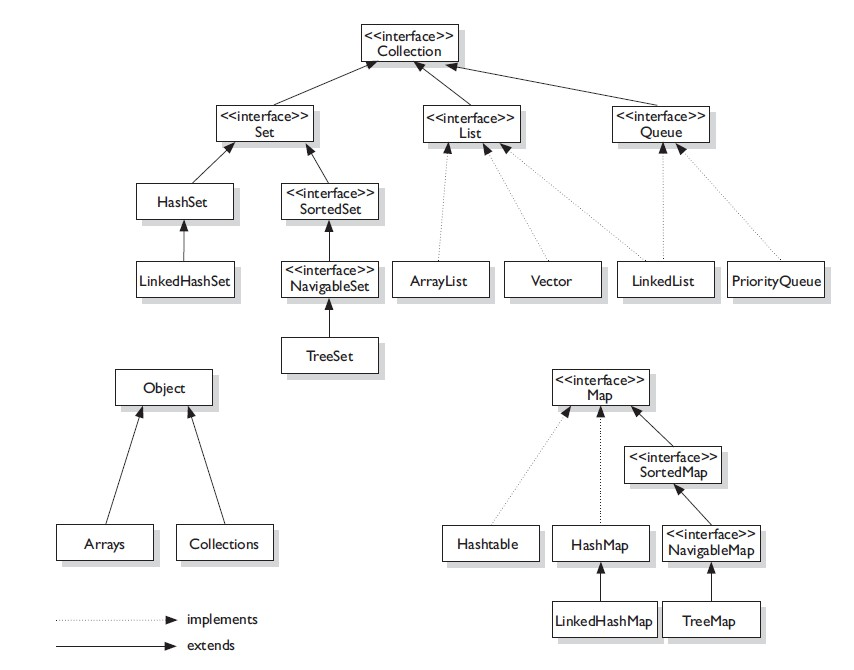
\includegraphics[scale=0.5]{Images/collections_hierarchy}
\end{center}

To make things a little more confusing, there are three overloaded uses of the 
word `collection':
\begin{description}
    \item[collection (lowercase `c')] Represents any of the data structures in 
    which objects are stored and iterated over
    \item[Collection (capital `C')] The \verb#java.util.Collection# interface 
    from which \verb#Set#, \verb#List# and \verb#Queue# extend (note extend and 
    not implement -- there are no direct implementations of \verb#Collection#)
    \item[Collections (capital `C' and ends with `s')] The 
    \verb#java.util.Collections# class that contains several \verb#static# 
    utility methods for use with collections
\end{description}

Collections come in four basic flavours:
\begin{itemize}
    \item Lists -- Lists of things (classes that implement \verb#List#)
    \item Sets -- Unique things (classes that implement \verb#Set#)
    \item Maps -- Things with a unique ID (classes that implement \verb#Map#)
    \item Queues -- Things arranged by the order in which thay are to be 
    processed
\end{itemize}
There are sub-flavours within these four:
\begin{itemize}
    \item Sorted
    \item Unsorted
    \item Ordered
    \item Unordered
\end{itemize}

\subsubsection{Ordered}
Allows iterating through the collection in a specific (non-random) order

\subsubsection{Sorted}
The order of the collection is determined according to some rules, known as the 
sort order. A sort order is unrelated to when an object is added to a 
collection, when it was last accessed or what `position' it is in. There is no 
natural ordering for objects unless one is provided through the 
\verb#Comparable# interface that defines how instances of one class can be 
compared to another. Aside from natural order as specified by the 
\verb#Comparable# interface, it is also possible to define other sort orders 
using the \verb#Comparator# interface

\subsection{List Interface}
A \verb#List# cares about the index. The one thing that \verb#List# has that 
non-lists don't have is a set of methods related to index. These key methods 
include things like \verb#get(int index)#, \verb#indexOf(Object o)#, 
\verb#add(int index, Object o)# and so on. All three \verb#List# 
implementations are ordered by index position -- a position that you determine 
either by setting an object at a specific index or by adding it without 
specifying a position, in which case the object is added to the end

\subsubsection{ArrayList}
An \verb#ArrayList# is like an expandable array. It provides fast iteration and 
random access. It is an ordered collection (by index) but is not sorted.  
\verb#ArrayList# implements the \verb#RandomAccess# marker interface

\subsubsection{Vector}
A \verb#Vector# is basically the same as an \verb#ArrayList# except that 
\verb#Vector# methods are synchronised. \verb#Vector# is the only class other 
than \verb#ArrayList# to implement the \verb#RandomAccess# marker interface

\subsubsection{LinkedList}
A \verb#LinkedList# is ordered by index position, like \verb#ArrayList# and 
\verb#Vector#, except that the elements are doubly-linked to one another. This 
linkage provides methods for adding and removing from the beginning or end, 
which suits stack or queue based collections. As of java 5, \verb#LinkedList# 
implements the \verb#java.util.Queue# interface and as such, supports the 
common queue methods: \verb#peek()#, \verb#poll()# and \verb#offer()#

\subsection{Set Interface}
A \verb#Set# cares about uniqueness -- it does not allow duplicates. The 
\verb#equals()# method is used to determine if two objects are identical (in 
which case only one can be in the set)

\subsubsection{HashSet}
A \verb#HashSet# is an unsorted, unordered \verb#Set#. It uses the hashcode of 
the object being inserted, so the more efficient the \verb#hashCode()# 
implementation, the better access performance provided

\subsubsection{LinkedHashSet}
A \verb#LinkedHashSet# is an ordered version of \verb#HashSet# that maintains a 
doubly-linked list across all elements. Objects are iterated in insertion order

\subsubsection{HashSet, LinkedHashSet and hashCode()}
Note that when using \verb#HashSet# or \verb#LinkedHashSet#, the objects you 
add to them must override \verb#hashCode()#. If they do not, the default 
\verb#Object.hashCode()# method will allow multiple objects that you might 
consider `meaningfully equivalent' to be added to your `no duplicates allowed' 
set

\subsubsection{TreeSet}
The \verb#TreeSet# is one of the two sorted collections (the other being 
\verb#TreeMap#). Elements are stored in ascending order, according to natural 
ordering. Optionally, you can construct a \verb#TreeSet# with a constructor 
that lets you give the collection your own rules for what the order should be 
(rather than relying on the ordering defined by the elements' class) by using a 
\verb#Comparable# or \verb#Comparator#. As of java 6, \verb#TreeSet# implements 
\verb#NavigableSet#

\subsection{Map Interface}
A \verb#Map# cares about unique identifiers. You map a unique key (the ID) to a 
specific value, where both the key and the value are objects. The \verb#Map# 
implementations let you do things like search for a value based on a key and 
ask for a collection of just the keys or values. Like \verb#Sets#, \verb#Map#s 
rely on the \verb#equals()# method to determine whether two keys are equivalent

\subsubsection{HashMap}
\verb#HashMap# gives  you an unsorted, unordered map. When you need a 
\verb#Map# and you don't care about the order, then \verb#HashMap# is suitable 
-- all other \verb#Map#s add a little more overhead. \verb#hashCode()# is used 
to determine where the keys land in the \verb#Map# and note that one 
\verb#null# key and multiple \verb#null# values are allowed

\subsubsection{Hashtable -- note lack of capital `t'}
\verb#Hashtable# is the synchronised counterpart of \verb#HashMap#. Note that a 
\verb#Hashtable# does not allow \verb#null# keys or values

\subsubsection{LinkedHashMap}
Like its \verb#Set# counterpart, \verb#LinkedHashSet#, \verb#LinkedHashMap# 
maintains insertion order (or optionally, access order). Although it will be 
slower than \verb#HashMap# for insertions and deletions, faster iteration can 
be expected

\subsubsection{TreeMap}
\verb#TreeMap# is a sorted \verb#Map#. Like \verb#TreeSet#, \verb#TreeMap# lets 
you define a custom sort order (via a \verb#Comparable# or \verb#Comparator#) 
when you construct it. Note that as of java 6, \verb#TreeMap# implements 
\verb#NavigableMap#

\subsection{Queue Interface}
Although other orders are possible, queues are typically thought of as FIFO 
(first-in, first-out). Queues support all of the standard \verb#Collection# 
methods and they also add methods to add, subtract and review queue elements

\subsubsection{PriorityQueue}
Introduced in java 5, a \verb#PriorityQueue# can be used to create a 
priority-in, priority-out queue. The elements are either ordered by natural 
ordering (in which case, the elements that are sorted first will be accessed 
first) or according to a \verb#Comparator#. In either case, the elements' 
ordering represents their relative priority. Note that since the 
\verb#LinkedList# class implements the \verb#Queue# interface, basic queues can 
be handled with a \verb#LinkedList#

\subsection{Summary of 11 of the 13 Concrete Collection-Oriented Classes}
\begin{center}
\begin{tabular}{llllp{4cm}p{4cm}l}
    \textbf{Class} & \textbf{List} & \textbf{Set} & \textbf{Map} & 
    \textbf{Ordered} & \textbf{Sorted} & Synchronised \\
    \hline
    \verb#ArrayList# & Y & & & By index & No & No \\
    \verb#Vector# & Y & & & By index & No & Yes \\
    \verb#LinkedList# & Y & & & By index & No & No \\
    \hline
    \verb#HashSet# & & Y & & No & No & No \\
    \verb#LinkedHashSet# & & Y & & By insertion order & No & No \\
    \verb#TreeSet# & & Y & & Sorted & By natural order or custom comparison 
    rules & No \\
    \hline
    \verb#HashMap# & & & Y & No & No & No \\
    \verb#Hashtable# & & & Y & No & No & Yes \\
    \verb#LinkedHashMap# & & & Y & By insertion order or last access order & No 
    & No \\
    \verb#TreeMap# & & & Y & Sorted & By natural order or custom comparison 
    rules & No \\
    \hline
    \verb#PriorityQueue# & & & & Sorted & By priority & No \\
\end{tabular}
\end{center}

\subsection{Using the Collections Framework}
\subsubsection{ArrayList Basics}
The \verb#java.util.ArrayList# is like an enhanced array. Some of the 
advantages over arrays are:
\begin{itemize}
    \item They can expand dynamically
    \item They provide more powerful insertion and search methods
\end{itemize}
A key design goal of the \verb#Collections# framework was to prvide rich 
functionality at the level of the main interfaces: \verb#List#, \verb#Set# and 
\verb#Map#. In practice, you'll usually instantiate an \verb#ArrayList# 
polymorphically:\\
\verb#List list = new ArrayList();# and as of java 5,
\verb#List<String> list = new ArrayList<String>();#

\subsubsection{Autoboxing with Collections}
In general, collections can hold \verb#Object#s but not primitives. Prior to 
java 5, you needed to wrap a primitive by hand before adding it to a 
collection. As of java 5, autoboxing will take care of the wrapping for you

\subsection{Sorting Collections and Arrays}
Both collections and arrays can be sorted and searched using methods in the API

\subsubsection{Sorting Collections}
\verb#ArrayList# does not provide any way to sort its contents, but the 
\verb#java.util.Collections# class provides static \verb#sort()# methods. The 
one-arg \verb#sort()# method takes a \verb#List# and the objects in the list 
must implement \verb#Comparable#. Note that there is also a two-arg 
\verb#sort()# method which takes a \verb#List# and a \verb#Comparator# to use 
for sorting

\subsubsection{The Comparable Interface}
The \verb#Comparable# interface is used by the 
\verb#java.util.Collections.sort()# and the \verb#java.util.Arrays.sort()# 
methods to sort \verb#List#s and arrays of objects. To implement 
\verb#Comparable#, a class must implement a single method --
\verb#int compareTo(Object anotherObject)#. The \verb#compareTo()# method 
returns an \verb#int# with the following characteristics:
\begin{itemize}
    \item negative -- if \verb#this < anotherObject#
    \item zero -- if \verb#this == anotherObject#
    \item positive -- if \verb#this > anotherObject#
\end{itemize}
The \verb#sort()# method uses \verb#compareTo()# to determine how the 
\verb#List# or object array should be sorted. An example of implementing 
\verb#Comparable# is:
\begin{verbatim}
    import java.lang.Comparable;    // NOTE: java.lang

    class DVDInfo implements Comparable<DVDInfo> {
        String title;
        public int compareTo(DVDInfo d) {
            return title.compareTo(d.getTitle());
        }
        public String getTitle() { return title; }
    }
\end{verbatim}
Note that prior to generics, \verb#Comparable# would have been implemented 
something like:
\begin{verbatim}
    import java.lang.Comparable;    // NOTE: java.lang

    class DVDInfo implements Comparable {
        String title;
        public int compareTo(Object o) { // takes an Object rather than a type
            DVDInfo d = (DVDInfo)o;
            return title.compareTo(d.getTitle());
        }
        public String getTitle() { return title; }
    }
\end{verbatim}
This approach is still legal but requires a cast (which should be checked to 
ensure it does not fail at runtime). Note that when overriding \verb#equals()#,
it must take an argument of type \verb#Object#, but when overriding 
\verb#compareTo()#, it should take advantage of generics and take an argument 
of the type you are comparing

\subsubsection{Sorting with Comparator}
There is an overloaded version of \verb#Collections.sort()# which takes both a 
list and a \verb#Comparator#. The \verb#Comparator# interface gives you the 
ability to sort a collection any number of ways. The other handy thing about 
the \verb#Comparator# interface is that you can use it to sort instances of any 
class -- even classes you can't modify (unlike the \verb#Comparable# interface, 
which requires that you modify the class whose instances you want to sort). An 
example is:
\begin{verbatim}
    import java.util.Comparator;    // NOTE: java.util
    class GenreSort implements Comparator<DVDInfo> {
        public int compare(DVDInfo one, DVDInfo two) {
            return one.getGenre().compareTo(two.getGenre());
        }
    }
\end{verbatim}
The \verb#Comparator.compare()# method returns an \verb#int# whose meaning is 
the same as the \verb#Comparable.compareTo()# method's return value

\subsubsection{Comparing Comparable and Comparator}
\begin{center}
\begin{tabular}{lp{6cm}p{6cm}}
    \textbf{Interface} & \textbf{java.lang.Comparable} & 
    \textbf{java.util.Comparator} \\
    \hline
    Key method & \verb#int objOne.compareTo(objTwo)# &
    \verb#int compare(objOne, objTwo)# \\
    \hline
    \multirow{3}{*}{Returns} & negative if \verb#objOne < objTwo# &
    \verb#negative if objOne < objTwo# \\
    & zero if \verb#objOne == objTwo# & zero if \verb#objOne == objTwo# \\
    & positive if \verb#objOne > objTwo# & positive if \verb#objOne > objTwo# 
    \\
    \hline
    Class Modification & Must modify the class whose instances you want to sort 
    & Build a separate class from the class whose instances you want to sort \\
    \hline
    Multiple Sorts & Only one sort can be created & Multiple sorts can be 
    created \\
    \hline
    Implemented by & Implemented frequently in the API by \verb#String#, 
    \verb#Wrapper#, \verb#Date#, \verb#Calendar#, \ldots & Designed to be 
    implemented to sort instances of third-party classes
\end{tabular}
\end{center}

\subsubsection{Sorting with the java.utils.Arrays Class}
Sorting arrays of objects is just like sorting collections of objects. The 
\verb#java.utils.Arrays.sort()# method provides the same interface as the 
\verb#Collections.sort()# method:
\begin{itemize}
    \item \verb#Arrays.sort(arrayToSort)#
    \item \verb#Arrays.sort(arrayToSort, Comparator)#
\end{itemize}
In addition, the \verb#Arrays.sort()# method is overloaded several times to 
provide sort methods for every type of primitive. The \verb#Arrays.sort()# 
methods that sort primitives always sort based on natural order. Don't be 
fooled by code which attempts to sort a primitive array using a 
\verb#Comparator#. Note that the \verb#sort()# methods for the 
\verb#Collections# and \verb#Arrays# class are \verb#static# methods, and they 
alter the objects they are sorting. Also note that when sorting an array or 
collection, the elements must all be mutually comparable. In general, objects 
of different types should not be considered mutually comparable, unless 
specifically stated

\subsection{Searching Arrays and Collections}
The \verb#java.util.Collections# and \verb#java.util.Arrays# class both provide 
methods that allow you to search for a specific element. When searching through 
collections or arrays, the following rules apply:
\begin{itemize}
    \item Searches are performed using the \verb#binarySearch()# method
    \item Successful searches return the \verb#int# index of the element being 
    searched
    \item Unsuccessful searches return an \verb#int# index that represents the 
    insertion point. The insertion point is the place in the collection/array 
    where the element would be inserted to keep it properly sorted. Since 
    positive return values and 0 indicate successful searches, the 
    \verb#binarySearch()# method uses negative numbers to indicate insertion 
    points. The actual insertion point in the collection.array can be 
    calculated as $-(returnValue + 1)$
    \item The collection/array being searched must be sorted prior to searching
    \item If you attempt to search a collection/array which is not sorted, the 
    results are unpredictable
    \item If the collection/array was sorted in natural order, it must be 
    searched in natural order (usually this is acomplished by not providing a 
    \verb#Comparator# as an argument to the \verb#binarySearch()# method)
    \item If the collection/array was sorted using a \verb#Comparator#, it must 
    be searched using the same \verb#Comparator#, which is passed as the second 
    argument to the \verb#binarySearch()# method. Note that \verb#Comparator#s 
    cannot be used when searching arrays of primitives
\end{itemize}
When working on searching and sorting questions, note that:
\begin{itemize}
    \item The collection/array must be sorted before searching
    \item If a \verb#Comparator# is used for either the search or the sort, it 
    must be used for both
\end{itemize}

\subsection{Converting Arrays to Lists and Lists to Arrays}
There are a couple of methods that allow you to convert arrays to \verb#List#s 
and \verb#List#s to arrays. The \verb#List# and \verb#Set# classes have 
\verb#toArray()# methods and the \verb#Arrays# class has an \verb#asList()# 
method. The \verb#Arrays.asList()# method copies an array into a \verb#List#.  
The API says, ``Returns a fixed-size list backed by the specified array 
(changes to the returned list `write through' to the array)''. When you use the 
\verb#asList()# method, the array and \verb#List# become joined so that when 
one is updated, the other is updated automatically.

There is nothing too fancy going on with the \verb#toArray# method. It comes in 
two flavours -- one that returns a new \verb#Object# array, and one that uses 
the array you provide as the destination

\subsection{Using Lists}
Remember that \verb#List#s are usually used to keep things in some kind of 
order. Lists allow you to override the ordering of elements by adding or 
removing elements at a specified index. Prior to java 5 and the enhanced 
\verb#for# loop, the most common way to examine a \verb#List# was through the 
use of an \verb#Iterator#. There are two \verb#Iterator# methods needed for the 
eam:
\begin{itemize}
    \item \verb#boolean hasNext()# -- Returns \verb#true# if there is at least 
    one more element in the collection being traversed. Invoking 
    \verb#hasNext()# does not move to the next element of the collection
    \item \verb#Object next()# -- Returns the next object in the collection and 
    moves forward to the element after the one just returned
\end{itemize}
Note that \verb#Iterator#s can utilise generics, removing the need for a cast 
when calling \verb#next()#:
\begin{verbatim}
    List<Dog> dogs = new ArrayList<Dog>();
    Iterator<Dog> iterator = dogs.iterator();
    while(iterator.hasNext()) {
        Dog d = iterator.next();
    }
\end{verbatim}
Note that if generics are not used when creating the iterator, then a cast is 
required when calling \verb#next()#

\subsection{Using Sets}
Remember that \verb#Set#s are used when you don't want any duplicates in a 
collection. If you attempt to add an element that already exists in the set, 
the duplicate element will not be added and the \verb#add()# method will return 
\verb#false#. Note that \verb#HashSet#s are not ordered -- iterating them is 
unpredictable. Note that whenever you want a colleciton to be sorted, its 
elements must be mutually comparable. Remember that unless otherwise specified, 
objects of different types are not mutually comparable

\subsection{Using Maps}
Remember that when you use a class that implements \verb#Map#, any classes that 
you use as a part of the keys for that map should override the \verb#equals()# 
and \verb#hashCode()# methods. Note that you only need to override them if you 
are interested in retrieving elements from the \verb#Map#. Note that enums 
override \verb#equals()# and \verb#hashCode()#. Note that in general, the more 
unique hashcodes a formula creates, the faster retrieval will be. Note that if 
an attibute of an object within a \verb#Map# is altered and the attribute is 
used as part of the \verb#hashCode()# method, then the object will not be found 
if a different hashcode results. There are two stages to retrieval from maps:
\begin{enumerate}
    \item Use \verb#hashCode()# to find the correct bucket
    \item Use \verb#equals()# to find the object in the bucket
\end{enumerate}

\subsection{Navigating (Searching) TreeSets and TreeMaps}
Java 6 introduced the \verb#java.util.NavigableSet# and 
\verb#java.util.NavigableMap# interfaces. For the purposes of the exam, you 
need to know how \verb#TreeSet# and \verb#TreeMap# implement these interfaces.  
For the purposes of the exam, the \verb#NavigableSet# methods related to 
navigation are \verb#lower()#, \verb#floor()#, \verb#ceiling()# and 
\verb#higher()#. The mostly parallel \verb#navigableMap# methods are 
\verb#lowerKey()#, \verb#floorKey()#, \verb#ceilingKey()# and 
\verb#higherKey()#. The difference between \verb#lower()# and \verb#floor()# is 
that \verb#lower()# returns the element less than the given element, and 
\verb#floor()# returns the element less than or equal to the given element.  
Similarly, \verb#higher()# returns the element greater than the given element, 
and \verb#ceiling()# returns the element greater than or equal to the given 
element

\subsection{Other Navigation Methods}
\subsubsection{Polling}
The idea of polling is that we want both to retrieve and remove an element from 
either the beginning or the end of a collection. In the case of \verb#TreeSet#, 
\verb#pollFirst()# returns and removes the first entry in the set, and 
\verb#pollLast()# returns and removes the last. Similarly, \verb#TreeMap# 
provides the \verb#pollFirstEntry()# and \verb#pollLastEntry()# to retrieve and 
remove key-value pairs

\subsubsection{Descending Order}
\verb#TreeSet.descendingSet()# and \verb#TreeMap.descendingMap()# can be used 
to return a collection in the reverse order of the collecton on which the 
method was invoked

\subsection{Important `Navigation' Related Methods}
\begin{center}
\begin{tabular}{ll}
    \textbf{Method} & \textbf{Description} \\
    \hline
    \verb#TreeSet.lower(e)# & Returns the highest element $<$ e \\
    \verb#TreeSet.floor(e)# & Returns the highest element $<=$ e \\
    \verb#TreeSet.ceiling(e)# & Returns the lowest element $>=$ e \\
    \verb#TreeSet.higher(e)# & Returns the lowest element $>$ e \\
    \verb#TreeSet.pollFirst()# & Returns and removes the first entry \\
    \verb#TreeSet.pollLast()# & Returns and removes the last entry \\
    \verb#TreeSet.descendingSet()# & Returns a \verb#NavigableSet# in reverse 
    order \\
    \hline
    \verb#TreeMap.lowerKey(e)# & Returns the highest key $<$ e \\
    \verb#TreeMap.floorKey(e)# & Returns the highest key $<=$ e \\
    \verb#TreeMap.pollFirstEntry()# & Returns and removes the first key-value 
    pair \\
    \verb#TreeMap.pollLastEntry()# & Returns and removes the list key-value 
    pair \\
    \verb#TreeMap.descendingMap()# & Returns a \verb#NavigableMap# in reverse 
    order \\
\end{tabular}
\end{center}

\subsection{Backed Collections}
Some of the classes in the \verb#java.util# package support the concept of 
`backed collections`. In these cases, when we add elements into either the 
original or modified collection, the new elements are automatically added to 
the other collection as long as the element is within the range of the modified 
collection. Note that an exception will be thrown if you attempt to add an 
out-of-range element to the modified collection. The \verb#TreeSet# and 
\verb#TreeMap# classes support backed collections via the following methods:
\begin{center}
\begin{tabular}{ll}
    \textbf{Method} & \textbf{Description} \\
    \hline
    \verb#headSet(e, b*)# & Returns a subset ending at and exclusive of element 
    \verb#e# \\
    \verb#tailSet(e, b*)# & Returns a subset starting at and inclusive of 
    element \verb#e# \\
    \verb#subSet(s, b*, e, b*)# & Returns a subset starting at \verb#s# and 
    ending just before element \verb#e# \\
    \hline
    \verb#headMap(k, b*)# & Returns a submap ending at and exclusive of key 
    \verb#k# \\
    \verb#tailMap(k, b*)# & Returns a submap starting at and inclusive of key 
    \verb#k# \\
    \verb#subMap(s, b*, e, b*)# & Returns a submap starting at \verb#s# and 
    ending just before key \verb#e# \\
\end{tabular}
\end{center}
*Note: These boolean arguments are optional. It they exist, it's a java 6 
method that allows you to specify whether the endpoint is exclusive, and these 
methods return a \verb#NavigableXxx#. If the boolean arguments do not exist, 
the method returns a \verb#SortedXxx#

\subsection{Using the PriorityQueue Class}
Unlike basic queue structures that are first-in, first-out by default, a 
\verb#PriorityQueue# orders its elements using a user-defined priority. The 
priority can be as simple as natural ordering (in which, for example, an entry 
of 1 would be a higher priority than an entry of 2). In addition, a 
\verb#PriorityQueue# can be ordered using a \verb#Comparator#, which lets you 
define any ordering you want. Queues have a few methods not found in other 
collection interfaces:
\begin{itemize}
    \item \verb#peek()# -- Returns (but does not remove) the highest priority 
    element in the \verb#PriorityQueue#
    \item \verb#poll()# -- Returns and removes the highest priority element in 
    the \verb#PriorityQueue#
    \item \verb#offer()# -- Adds elements to the \verb#PriorityQueue#
\end{itemize}

\subsection{Method Overview for Arrays and Collections}
\begin{center}
\begin{tabular}{lp{0.4\textwidth}}
    \textbf{Key Methods in java.util.Arrays} & \textbf{Description} \\
    \hline
    \verb#static List asList(T[])# & Convert an array to a \verb#List# (and 
    bind them) \\
    \hline
    \verb#static int binarySearch(Object[], key)# & 
    \multirow{2}{0.4\textwidth}{Search a sorted array for a given value, return 
    an index or insertion point} \\
    \verb#static int binarySearch(primitive[], key)# & \\
    \hline
    \verb#static int binarySearch(T[], key, Comparator)# & Search a 
    \verb#Comparator#-sorted array for a value \\
    \hline
    \verb#static boolean equals(Object[], Object[])# & 
    \multirow{2}{0.4\textwidth}{Compare two arrays to determine if their 
    contents are equal} \\
    \verb#static boolean equals(primitive[], primitive[])# & \\
    \hline
    \verb#static void sort(Object[])# & \multirow{2}{0.4\textwidth}{Sort the 
    elements of an array by natural order} \\
    \verb#static void sort(primitive[])# & \\
    \hline
    \verb#static void sort(T[], Comparator)# & Sort the elemetns of an array 
    using a \verb#Comparator# \\
    \hline
    \verb#static String toString(Object[])# & 
    \multirow{2}{0.4\textwidth}{Create a String containing the contents of an 
    array} \\
    \verb#static String toString(primitive[])# & \\
\end{tabular}

\begin{tabular}{lp{0.4\textwidth}}
    \textbf{Key Methods in java.util.Collections} & \textbf{Description} \\
    \hline
    \verb#static int binarySearch(List, key)# & 
    \multirow{2}{0.4\textwidth}{Search a sorted List for a given value, return 
    an index or insertion point} \\
    \verb#static int binarySearch(List, key, Comparator)# & \\
    \hline
    \verb#static void reverse(List)# & Reverse the order of elements in a 
    \verb#List# \\
    \hline
    \verb#static Comparator reverseOrder()# & 
    \multirow{2}{0.4\textwidth}{Returns a Comparator that sorts the reverse of 
    the collection's current sort sequence} \\
    \verb#static Comparator reverseOrder(Comparator)# & \\
    \hline
    \verb#static void sort(List)# & \multirow{2}{0.4\textwidth}{Sort a List by 
    natural order or by a Comparator} \\
    \verb#static void sort(List, Comparator)# & \\
\end{tabular}
\end{center}

\subsection{Method Overview for List, Set and Map}
\begin{center}
\begin{tabular}{llllp{0.3\textwidth}}
    \textbf{Key Interface Methods} & \textbf{List} & \textbf{Set} & 
    \textbf{Map} & \textbf{Description} \\
    \hline
    \verb#boolean add(element)# & Y & Y & & \multirow{2}{0.3\textwidth}{Add an 
    element. For Lists, optionally add at an index} \\
    \verb#boolean add(index, element)# & Y & & & \\
    \hline
    \verb#boolean contains(Object)# & Y & Y & & 
    \multirow{3}{0.3\textwidth}{Search a collection for an Object (or 
    optionally for Maps, a key)} \\
    \verb#boolean containsKey(Object key)# & & & Y & \\
    \verb#boolean containsValue(Object value)# & & & Y & \\
    \hline
    \verb#Object get(index)# & Y & & & \multirow{2}{0.3\textwidth}{Get an 
    object from a collection via an index or key} \\
    \verb#Object get(key)# & & & Y & \\
    \hline
    \verb#int indexOf(Object)# & Y & & & Get the location of an Object in a 
    List \\
    \hline
    \verb#Iterator iterator()# & Y & Y & & Get an Iterator for a List or Set \\
    \hline
    \verb#Set keySet()# & & & Y & Return a Set containing a Map's keys \\
    \hline
    \verb#put(key, value)# & & & Y & Add a key/value pair to a Map \\
    \hline
    \verb#remove(index)# & Y & & & \multirow{3}{0.3\textwidth}{Remove an 
    element via an index, value or key} \\
    \verb#remove(Object)# & Y & Y & & \\
    \verb#remove(key)# & & & Y & \\
    \hline
    \verb#int size()# & Y & Y & Y & Returns the number of elements in a 
    collection \\
    \hline
    \verb#Object[] toArray()# & Y & Y & & \multirow{2}{0.3\textwidth}{Return an 
    array containing the elements of the collection} \\
    \verb#T[] toArray(T[])# & Y & Y & & \\
    \hline
\end{tabular}
\end{center}

\subsection{Note on Character Sort Order}
Remember that spaces sort before characters and that uppercase characters sort 
before lowercase characters

\subsection{Generic Types}
Remember that before java 5 there was no syntax for declaring a type safe 
collection. To declare an \verb#ArrayList# of \verb#String#s you said, 
\verb#ArrayList list = new ArrayList()# or the polymorphic equivalent, 
\verb#List list = new ArrayList()#. There was no syntax that let you specify 
that \verb#list# will hold only \verb#String#s. With no way to specify a type 
for the \verb#ArrayList#, the compiler could not enforce that you put only 
things of the specified type into \verb#list#. As of java 5, we can use 
generics, and while they are not only for making type safe collections, that is 
just about all most developers use them for

\subsubsection{The Legacy Way to do Collections}
\begin{verbatim}
    List list = new ArrayList();    // can't declare type
    list.add("Kevin");              // list can hold Strings
    list.add(new Dog());            // list can hold Dogs
    list.add(new Integer(42));      // list can hold Integers...
\end{verbatim}
A non-generic collection can hold any kind of object (i.e. anything which is 
not a primitive). Since the collection could hold anything, the methods that 
get objects out of the collection had a return type of \verb#java.lang.Object#.  
Which meant that an explicit cast was required which could potentially fail at 
runtime:
\begin{verbatim}
    String s = (String)list.get(0);
\end{verbatim}
Generics address both the adding and retrieving problem described by enforceing 
the type of the collection:
\begin{verbatim}
    List<String> list = new ArrayList<String>();    // declare type
    list.add("Kevin");                              // no problem
    list.add(new Dog());                            // compilation failure
\end{verbatim}
Since the compiler knows the type of the collection, no cast is required when 
retrieving elements:
\begin{verbatim}
    String s = list.get(0);
\end{verbatim}
We can also use the collection in a for-each loop (\verb#for(String s : list)#) 
without any problems and methods can accept typed collections as arguments and 
return them too.

Note that a list of type \verb#List list = new ArrayList()# is almost identical 
to \verb#List<Object> list = new ArrayList<Object>()#. Note that the type in 
angle brackets is referred to as either `parameterised type', `type parameter', 
or just `type'

\subsubsection{Generics and Legacy Code}
For the exam, you'll need to know how to update non-generic code to make it 
generic. You just add a type in angle brackets (\verb#<>#) immediately 
following the collection type in both the variable declaration and the 
constructor call, including any place you declare a variable (i.e. method 
arguments and return types too). Note that it is not necessary to remove any 
explicit casts when retrieving elements from the collection (since it is 
effectively a no-op) 

\subsubsection{Mixing Generic and Non-Generic Collections}
The compiler will generate warnings if there is a chance a type safe collection 
could be modified by non-type-safe code. Generics are strictly compile-time 
protection. The compiler uses generic type information (the \verb#<type># in 
the angle brackets) to make sure that your code does not put the wrong things 
into a collection, and that you do not assign what you get from a collection to 
the wrong reference type. However, none of this protection exists at runtime.  
The fact is, you do not need runtime protection until you start mixing up 
generic and non-generic code.

On the exam, you must be able to recognise when you are compiling code that 
will produce warnings but still compile. Any code that compiles (even with 
warnings) will run. No type violations will be caught at runtime by the JVM, 
until those type violations mess with your code in some other way. In other 
words, the act of adding a \verb#String# to an \verb#<Integer># list will not 
fail at runtime until you try to treat that String-you-think-is-an-Integer as 
an \verb#Integer#.

When using legacy (non-type safe) collections, watch out for unboxing problems.  
If you declare a non-generic collection, the \verb#get()# method always returns 
a reference of type \verb#java.lang.Object#. Remember that unboxing cannot 
convert an \verb#Object# to a primitive, even if that \verb#Object# reference 
refers to a wrapped primitive. Unboxing converts only from a wrapper class 
reference to a primitive:
\begin{verbatim}
    List list = new ArrayList();
    list.add(43);
    int x = (Integer)list.get(0);   // cast required

    List<Integer> list2 = new ArrayList<Integer>();
    list2.add(43);
    int x2 = list2.get(0);          // cast not required
\end{verbatim}

\subsubsection{Polymorphism and Generics}
If you declare \verb#List<Foo> foo# then whatever you assign to the foo 
reference must be of the generic type \verb#<Foo># -- not a subtype of 
\verb#<Foo>#, not a supertype of \verb#<Foo>#, just \verb#<Foo>#. These are 
incorrect:
\begin{verbatim}
    List<Object> list = new ArrayList<Dog>();
    List<Number> list2 = new ArrayList<Integer>();
\end{verbatim}
These are fine:
\begin{verbatim}
    List<Dog> list = new ArrayList<Dog>();
    List<Integer> list2 = new ArrayList<Integer>();
\end{verbatim}
Note that this is different to how arrays behave, where you can do this: 
\verb#Object[] list = new Integer[3];# but not this:
\verb#List<Object> list = new ArrayList<Integer>();#

\subsubsection{Generic Methods}
When a method accepts an \verb#ArrayList<Animal>#, it will not be able to 
accept a collection of any \verb#Animal# subtype (eg. \verb#ArrayList<Dog>#).  
The reason for this is that within the method, the parameter is of type 
\verb#ArrayList<Animal>#, and that means you could put any kind of 
\verb#Animal# into the collection. There is simply no way for the compiler to 
stop you from putting a \verb#Dog# into a \verb#List# that was originally 
declared as \verb#<Cat>#, but is now referenced from the \verb#<Animal># 
parameter.

This is the scenario we are trying to prevent, regardless of whether we are 
using an array or an \verb#ArrayList#. The difference is that the compiler lets 
you get away with it for arrays, but not for generic collections. The reason 
you can get away with it for arrays is that there is a runtime exception 
\verb#ArrayStoreException# that will prevent you from putting the wrong type of 
object into an array.

However, there is no equivalent exception for generics, due to type erasure. In 
other words, at runtime the JVM knows the type of arrays, but does not know the 
type of a collection. All the generic type information is removed during 
compilation, so by the time it gets to the JVM, there is simply no way to 
recognise the disaster of putting a \verb#Cat# into an \verb#ArrayList<Dog># 
and vice versa (and it becomes exactly like the problems associated with using 
legacy, non-type safe code).

The generic type of an object is always the same as the generic type declared 
on the reference. \verb#List<Dog># can only refer to collections that are 
subtypes of \verb#List# which were instantiated as generic type \verb#<Dog>#.

There is a mechanism to tell the compiler that a method can accept any generic 
subtype of the declared argument type becasue the method will not add anything 
to the collection. This mechanism is the wildcard \verb#<?># For example, 
\verb#void addAnimal(List<? extends Animal> animals) {}#. 

The \verb#List<? extends Animal># means that \verb#addAnimal# can accept any 
collection which is a subtype of \verb#List#, having a generic type which:
\begin{itemize}
    \item is a subclass (abstract or concrete) of \verb#Animal#, or
    \item implements the interface \verb#Animal#
\end{itemize}
In other words, the keyword \verb#extends# in the context of a wildcard 
represents both subclasses and interface implementation. There is no
\verb#<?  implements Serializable># syntax for example. If you want to declare 
a method that accepts anything that implements \verb#Serializable#, you would 
use \verb#<? extends Serializable>#. So when \verb#extends# is used as part of 
a wildcard, think Is-A

There is another scenario where you can use a wildcard and still add to the 
collection in a safe way -- using the keyword \verb#super#:
\verb#void addAnimal(List<? super Dog> animals) {}#. When you use the
\verb#<? super ...># syntax, you are telling the compiler that you can accept 
the type on the right-hand-side of \verb#super# or any of its supertypes, since 
a collection declared as a supertype will be able to accept a subtype as an 
element. So the \verb#super# keyword in wildcard notation lets you have a 
restricted, yet extendable collection. Note that \verb#List<? extends Object># 
and \verb#List<?># are identical.

Keep in mind that wildcards can be used only for reference declarations 
(including arguments, variables, return types, and so on). They can not be used 
as the type parameter when you create a typed collection

\subsubsection{Generic Declarations}
The API tells you when a parameterised type is required. For example, the API 
declaration for the \verb#java.util.List# interface is: \verb#public interface List<E>#. The \verb#<E># is a placeholder for the type you pass in. The use of 
the letter `E' is just a convention -- any valid identifier would work, but 
here, `E' stands for `Element', and it is only used when the template is a 
collection. The other main convention is `T' (for `Type'), which is used for 
anything other than a collection. When you see a generic class or interface, 
pick a type parameter and do a mental find and replace on each occurrence of 
the type parameter. An example of a generic class is:
\begin{verbatim}
    public class TestGenerics<T> {
        T anInstance;                       // instance variable type
        T[] anArrayOfTs;                    // array type

        TestGenerics(T anInstance) {        // argument type
            this.aninstance = anInstance;
        }

        T getT() {                          // return type
            return anInstance;
        }
    }
\end{verbatim}
Note that you can use multiple parameterised types in a single class 
definition:
\begin{verbatim}
    public class UseTwo<O, T> {
        O one;
        T two;

        UseTwo(O one, T two) {
            this.one = one;
            this.two = two;
        }

        O getOne() { return one; }
        T getTwo() { return two; }

        public static void main(String[] args) {
            UseTwo<String, Integer> useTwo = new UseTwo<String, Integer>("a", 1);
            String s = useTwo.getOne();
            Integer i = useTwo.getTwo();
        }
    }
\end{verbatim}
Note that you can use a form of wildcard notation in a class definition, to 
specify a range (called `bounds') for the type that can be used for the type 
parameter:
\begin{verbatim}
    class AnimalHolder<T extends Animal> {     // use 'T' rather than '?'
        T animal;

        public static void main(String[] args) {
            AnimalHolder<Dog> dogHolder = new AnimalHolder<Dog>();  // ok
            AnimalHolder<Integer> x = new AnimalHolder<Integer>();  // compilation failure
        }
    }
\end{verbatim}

\subsubsection{Creating Generic Methods}
Using a generic type, you can declare a method with a specific type and then 
get the type information based on the type of the object passed to the method:
\begin{verbatim}
    import java.util.*;
    class CreateAnArrayList {                   // not generic
        public <T> void makeArrayList(T t) {    // NOTE: generic type must be 
                                                // declared before method return
                                                // type
            List<T> list = new ArrayList<T>();
            list.add(t);
        }
    }
\end{verbatim}

The strangest thing about generic methods is that you must declare the type 
variable before the return type of the method. The \verb#<T># before 
\verb#void# simply defines what \verb#T# is before you use it as a type in the 
argument. You must declare the type this way unless it is specified for the 
class. In \verb#CreateAnArrayList#, the class is not generic, so there is no 
type parameter which can be used in \verb#makeArrayList#. Note that in the case 
of constructors, the type parameter must be declared before the constructor 
name (since there is no return type).

You can put boundaries on the type you declare, for example, if you want to 
restrict the \verb#makeArrayList()# method to only \verb#Number# or its 
subtypes: \verb#public <T extends Number> void makeArrayList(T t) {}#
